
======================================================================
starting package maintenance...
installation directory: "C:\Users\Bernardo Goncalves\AppData\Local\Programs\MiKTeX"
package repository: https://mirror.kku.ac.th/CTAN/systems/win32/miktex/tm/packages/
package repository digest: bc26c9dcac319ee10e5af84d3734de2b
going to download 69253 bytes
going to install 43 file(s) (1 package(s))
downloading https://mirror.kku.ac.th/CTAN/systems/win32/miktex/tm/packages/latexindent.tar.lzma...
0.07 MB, 0.24 Mbit/s
extracting files from latexindent.tar.lzma...
======================================================================
\documentclass{article}

% Language setting
% Replace `english' with e.g. `spanish' to change the document language
\usepackage[english]{babel}

% Set page size and margins
% Replace `letterpaper' with `a4paper' for UK/EU standard size
\usepackage[a4paper,top=2cm,bottom=2cm,left=3cm,right=3cm,marginparwidth=1.75cm]{geometry}

% Useful packages
\usepackage{amsmath}
\usepackage{graphicx}
\usepackage{subcaption}
\usepackage{booktabs}
\usepackage{multirow}
\usepackage{array}

\usepackage[colorlinks=true, allcolors=blue]{hyperref}

\title{Detecting adrenal lesions using machine learning - a state of the art}
\author{Bernardo Gonçalves - 58885 - Doctoral program in Biomedical Engineering}

\begin{document}
\maketitle

\section{Adrenal Glands and Adrenal Lesions}

\subsection{Anatomy, physiology and pathophysiology (CHANGE)}

The adrenal glands, or suprarenal glands, are two small glands located on top of the kidneys.  Each has a body and two limbs \cite{Baba2012}, and weights about 5g \cite{brit}. Figure \ref{fig:adrenal_ana} shows the localisation and anatomy of the adrenal glands. A slice of the right adrenal gland can be linear, comma or V-shaped. On the other hand, the left adrenal is triangular or Y-shaped.

\begin{figure}
    \centering
    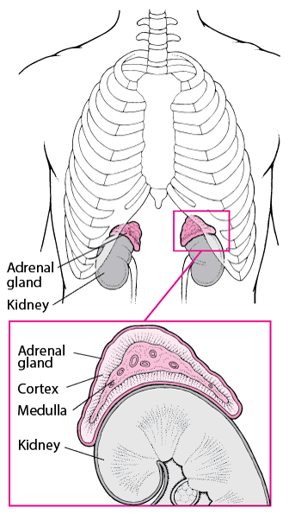
\includegraphics[scale=0.6]{figures/adrenal_anatomy.png}
    \caption{Adrenal localization and anatomy. From \textbf{ADD REFERENCE}}
    \label{fig:adrenal_ana}
\end{figure}

The adrenal gland has two different regions: the adrenal cortex and the adrenal medulla. The adrenal medulla is the inner region of the gland and is derived from the mesoderm \cite{Baba2012}. This region is responsible for the production of epinephrine and norepinephrine, which stimulates the fight-or-flight response \cite{openstax}. The adrenal cortex is the outer region of the gland and is derived from neural crest cells \cite{Baba2012}. This region is responsible for the production of cortisol, corticosterone, and cortisone, which increase blood glucose levels, and the production of aldosterone, which increases the level of sodium in the blood \cite{openstax}.

The adrenal glands can be affected by a wide variety of benign and malignant lesions. It is estimated that approximately 6\% of the population has them \cite{Panda2015}. These lesions can be primary if they originated in the glands themselves (cortex or medulla) or secondary if they have another origin. Primary lesions can be functional if they produce hormones \cite{Panda2015}. Table <PUT TAB 1> presents an overview of the adrenal lesions. The most common adrenal lesions are adenomas. Adenomas are often non-functional and remain asymptomatic, being discovered incidentally \cite{Wang2018}. Adenomas are, in most cases, non-functional and remain asymptomatic, being discovered incidentally \cite{Platzek2019}. Adrenocortical carcinoma is a rare lesion although it is the most common primary malignant adrenal lesion. This lesion affects children in their first decade and adults in their fourth and fifth decades \cite{Panda2015}. Also, the adrenals are a frequent location of metastases \cite{Platzek2019}.

Functional lesions can cause endocrines syndromes, such as Conn and Cushing syndrome. The Cushing syndrome or hypercortisolism is caused by elevated values of cortisol and it is associated with adrenal adenomas, mostly. Nevertheless, adrenocortical carcinomas or pheochromocytomas can also cause Cushing syndrome. This syndrome is defined by symptoms like obesity, rounded face, abnormal skin pigmentation, muscle weakness, hypertension, diabetes, and others. On the other hand, the Conn syndrome or primary aldosteronism is related to the excessive production of aldosterone. The most common symptoms of this syndrome are sodium retention, plasma renin suppression, hypertension, cardiovascular damage, and increased potassium excretion. Like the Conn syndrome, this syndrome is commonly caused by adrenal adenomas.  .  In opposition to the above-mentioned syndromes, the Addison disease is caused by adrenal insufficiency, which can be caused by malignant lesions. Patients with this disease can experience weight loss, weakness, fatigue, gastrointestinal upset, orthostatic hypotension, and abnormal skin pigmentation. These symptoms can evolve into dehydration, shock, hyperkalaemia (high potassium), and hyponatremia (high sodium) when entering acute adrenal insufficiency \cite{Wang2018}.

\begin{figure}
    \centering
    \begin{subfigure}[b]{0.45\textwidth}
        \centering
        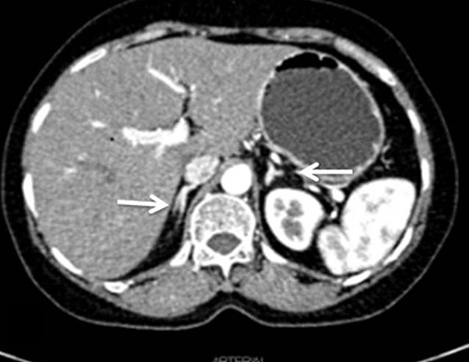
\includegraphics[width=\textwidth]{figures/CT_adrenal_enhanced.png}
        \caption{Adrenal glands in a contrast-enhanced CT axial slice in arterial phase. Due to the high level of retroperitoneal fat both glands are enhanced in this image slice. Reprinted from \cite{Panda2015}}
        \label{fig:adrenal_ct}
    \end{subfigure}
    \hfill
    \begin{subfigure}[b]{0.45\textwidth}
        \centering
        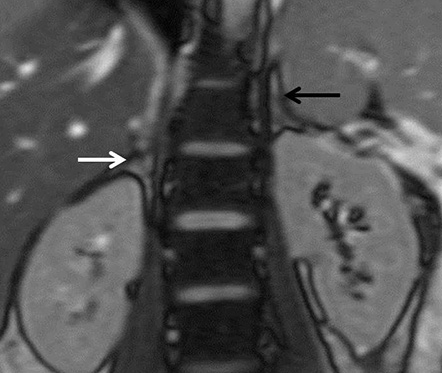
\includegraphics[width=\textwidth]{figures/MRI_adrenal.png}
        \caption{Adrenal glands in a MR CSI coronal slice. Both glands have a intermediate signal intensity. Reprinted from \cite{Panda2015} }
        \label{fig:adrenal_mri}
    \end{subfigure}
    \caption{Both figures show the y and v shaped adrenal glands. The arrows indicate the localization of the glands.}
    \label{fig:three graphs}
\end{figure}

\subsection{Adrenals Imaging}

Structural medical imaging techniques are decisive to detect and characterize adrenal lesions and complementary to functional imaging and endocrine evaluation in the assessment of functional lesions. Imaging techniques can also rule out invasive interventions. The most used imaging techniques to evaluate the adrenal glands are Computed Tomography (CT) and Magnetic Resonance Imaging (MRI). The Ultrasonography (USG) despite being a common method to assess abdominal pathologies, is not a good method to perceive retroperitoneal (back of the peritoneum) structures like the adrenals \cite{Panda2015}. Both Figures <ref FIG 2> and <REF FIG 3> show the V and Y-shaped normal glands. Figure <ref FIG 2> is an axial contrast-enhanced CT image in the arterial phase where both glands are enhanced due to the high retroperitoneal fat content. Figure <REF FIG 3> is a coronal MR Chemical Shift Image (CSI) out-of-phase showing normal adrenal glands also.

Commonly, non-functional lesions do not require any treatment and, for that reason it is crucial to differentiate between adenomas and non-adenomas \cite{Platzek2019}. Adrenal adenomas have less than 1 cm in diameter, usually and they can be lipid-rich or lipid-poor \cite{Panda2015}. About 70-80 \% of the adenomas are lipid-rich in contrast with the malignant lesions \cite{Platzek2019}. This results in a 20-30 \% overlap between adenomas and malignant lesions in terms of intracytoplasmic lipid content \cite{Israel2004}. Lipid-rich adenomas can be easily detected using unenhanced CT (less than 10 HU) \cite{Panda2015} or CSI \cite{Platzek2019}. However, lipid-poor adenomas cannot be correctly characterised by unenhanced CT \cite{Israel2004}. In these cases, CSI presents itself as a better solution because of its improved sensitivity to low levels of lipid content and therefore it can detect 62-67\% of the adenomas uncharacterised by CT \cite{Israel2004}. CSI is a fat-suppression technique that originates two sets of images: in-phase (IP) and out-of-phase (OP) images. In OP images the signal is the difference between the signals of water and fat molecules. In IP images the signal of both water and fat is added. Thus, there is a significant suppression of signal from IP to OP images in lipid-rich lesions \cite{Jahanvi2021}. OP images are characterised by the so-called India ink artefact that is a signal void in the margins of fatty and normal tissues \cite{Jahanvi2021}, creating a darker boundary in lipid-rich lesions like most adenomas. \cite{Platzek2019} performed a metanalysis with 1280 lesions (859 adenomas, 421 non-adenomas) and documented a sensitivity of 94\% and specificity of 95\% detecting adrenal adenomas. The same study states the importance of using Dynamic Contrast-Enhanced (DCE) MRI to improve the detection performance of lipid-poor adenomas. Adenomas present a signal increase in the arterial phase and a rapid washout \cite{Chung2001}.

\section{Differential diagnosis of adrenal lesions - current medical approach}

\subsection{Current procedure}

\subsection{Main limitations and setbacks}

\section{Differential diagnosis of adrenal lesions - machine learning approach}

\subsection{Research scope}

The presented state of the art was accomplished using the following research string: \textit{(adrenal or suprarenal) AND (CT OR "computed tomography" OR MRI OR "magnetic resonance imaging" OR "MRI scan" OR "nuclear magnetic resonance" OR "magnetic resonance" OR NMR ) AND ("deep learning" OR "convolutional networks" OR CNN OR "neural networks" OR convolutional OR DNN OR SVM OR "Support vector machine" OR "decision tree" OR "machine learning" ) AND (Classif* or diagnos* or dete* or locali* or "lesion segmentation")}. The analysed papers were published between 2017 and 2022. \textbf{Pubmed and Web Of Science (cite this)} were the used academic search engines.
The focus of this research is on works that apply machine learning (ML) methods to extract insights of abdominal Computed Tomography (CT) or Magnetic Resonance (MR) images to perform differential diagnosis of the adrenal lesions. We aim to answer the following questions:
\begin{enumerate}
    \item What is the relevance of using machine learning methods to differentiate adrenal lesions?
    \item The diagnosis performance is better with CT and RM images?
    \item What are the common used machine learning methods?
    \item What are the main limitations when performing differential diagnosis of adrenal lesions with ML?
    \item Can Deep Learning be presented as solution to differential diagnosis of adrenal lesions?
\end{enumerate}
All papers retrieved by the above mentioned research string that do not fall in this scope were excluded.
In total 21 papers were found and 3 were excluded. Thus, 18 papers were left to analyse and produce this review.

\subsection{Group A - Adenomas vs other lesions}

\begin{table}[]
    \centering
    \begin{tabular}{ccccc}\toprule
        \multirow{2}{*}{\textbf{Reference}} & \multirow{2}{*}{\textbf{Image Modality}} & \multicolumn{3}{c}{\textbf{Sample Size (lesions)}}
        \\\cmidrule(lr){3-5}
                                            &                                          & \textbf{Total}                                     & \textbf{Adenomas} & \textbf{Other} \\\midrule
        \cite{Tu2018}                       & U-CT                                     & 76                                                 & 36                & 40             \\
        \cite{Yi20181}                      & U/CE-CT                                  & 110                                                & 80                & 30             \\
        \cite{Yi2018}                       & U-CT                                     & 265                                                & 181               & 84             \\
        \cite{Elmohr2019}                   & CE-CT                                    & 54                                                 & 25                & 29             \\
        \cite{Torresan2021}                 & U/CE-CT                                  & 19                                                 & 9                 & 10             \\
        \cite{Kusunoki2022}                 & U/CE-CT                                  & 115                                                & 83                & 32             \\
        \cite{Liu2022}                      & U/CE-CT                                  & 280                                                & 188               & 92             \\
        \cite{Ho2019}                       & U/CE-CT; T1W-OP/IP MRI                   & 23                                                 & 15                & 8              \\
        \cite{Liu2021}                      & T1W-OP/IP; T2W MRI                       & 60                                                 & 40                & 20             \\
        \cite{Schieda2017}                  & T1W-OP/IP; T2W MRI                       & 44                                                 & 29                & 15             \\
        \cite{Tu2020}                       & T1W-OP/IP; T2W MRI                       & 63                                                 & 23                & 40             \\
        \cite{Romeo2018}                    & T1W-OP/IP; T2W MRI                       & 60                                                 & 40                & 20
        \\\bottomrule
    \end{tabular}
    \caption{Dataset Details for each article in the Group A. CT: Computed Tomography; U: Unenhanced; CE: Contrast Enhanced; MRI: Magnetic Resonance Imaging; OP: Out-of-phase; IP: In-phase; T1W: T1-weighted; T2W: T2-weighted}
    \label{tab:data_A}
\end{table}

\begin{table}[]
    \centering
    \begin{tabular}{cccccc}\toprule
        \multirow{2}{*}{\textbf{Reference}} & \multirow{2}{*}{\textbf{Type}} & \multirow{2}{*}{\textbf{Classification Model}} & \multirow{2}{*}{\textbf{ROI}} & \multirow{2}{*}{\textbf{Features}} \\
        \\\midrule
        \cite{Tu2018}                       & ML                             & LogReg                                         & Manual                        & $1^{st}$                           \\
        \cite{Yi20181}                      & ML                             & LogReg                                         & Manual                        & $1^{st}$, $2^{nd}$                 \\
        \cite{Yi2018}                       & ML                             & LASSO-LogReg                                   & Manual                        & $1^{st}$, $2^{nd}$                 \\
        \cite{Elmohr2019}                   & ML                             & RanFor; LogREg                                 & Manual                        & $1^{st}$, $2^{nd}$, shape          \\
        \cite{Torresan2021}                 & ML                             & K-Means                                        & Manual                        & $1^{st}$, $2^{nd}$                 \\
        \cite{Kusunoki2022}                 & DL                             & DCNN                                           & Manual                        & -                                  \\
        \cite{Liu2022}                      & ML                             & LinReg; SVM; RanFor                            & Manual                        & $1^{st}$; clinical                 \\
        \cite{Ho2019}                       & ML                             & LogReg                                         & Manual                        & $1^{st}$, $2^{nd}$, shape          \\
        \cite{Liu2021}                      & ML                             & SVM                                            & Manual                        & $1^{st}$                           \\
        \cite{Schieda2017}                  & ML                             & LogReg                                         & Manual                        & $1^{st}$                           \\
        \cite{Tu2020}                       & ML                             & LogReg                                         & Manual                        & $1^{st}$, shape                    \\
        \cite{Romeo2018}                    & ML                             & DecTre                                         & Manual                        & $1^{st}$, $2^{nd}$                 \\
        \bottomrule
    \end{tabular}
    \caption{Modelling Details  for each article in the Group A. ML: Traditional Machine Learning models; DL: Deep Learning models; LogReg: Logistic Regression; LASSO: Least Absolute Shrinkage and Selection Operator; DecTre: Decision Tree; RanFor: Random Forest; PCA: Principal Components Analysis; SVM: Support Vector Machine; $1^{st}$, $2^{nd}$, higher: first, second, higher order statistics, respectively; shape: shape-based features}
    \label{tab:model_A}
\end{table}

\begin{table}[]
    \centering
    \begin{tabular}{cccccc}\toprule
        \multirow{2}{*}{\textbf{Reference}} & \multirow{2}{*}{\textbf{Specificity - \%}} & \multirow{2}{*}{\textbf{Sensitivity - \%}} & \multirow{2}{*}{\textbf{Accuracy - \%}} & \multirow{2}{*}{\textbf{AUC - \%}} \\
        \\\midrule
        \cite{Tu2018}                       & 75.0                                       & 47.5                                       & 60.5                                    & 65.0                               \\
        \cite{Yi20181}                      & 97.5                                       & 86.2                                       & 94.4                                    & 95.2                               \\
        \cite{Yi2018}                       & 90.3                                       & 95.5                                       & 92.0                                    & 95.7                               \\
        \cite{Elmohr2019}                   & 83.0                                       & 81.0                                       & 82.0                                    & 89.0                               \\
        \cite{Torresan2021}                 & 90.0                                       & 87.5                                       & 88.9                                    & -                                  \\
        \cite{Kusunoki2022}                 & 96.0                                       & 87.0                                       & 94.0                                    & -                                  \\
        \cite{Liu2022}                      & 86.6                                       & 89.2                                       & 87.5                                    & -                                  \\
        \cite{Ho2019}                       & -                                          & -                                          & 80.0                                    & -                                  \\
        \cite{Liu2021}                      & -                                          & -                                          & 85.0                                    & 91.7                               \\
        \cite{Schieda2017}                  & 86.2                                       & 93.3                                       & 88.6                                    & 97.0                               \\
        \cite{Tu2020}                       & 100                                        & 75.0                                       & 84.1                                    & -                                  \\
        \cite{Romeo2018}                    & -                                          & -                                          & 80.0                                    & -                                  \\
        \bottomrule
    \end{tabular}
    \caption{Model metrics for each article in the Group A. AUC: Area Under the ROC Curve.}
    \label{tab:res_A}
\end{table}

\subsection{Malign vs benign lesions}

\begin{table}[]
    \centering
    \begin{tabular}{ccccc}\toprule
        \multirow{2}{*}{\textbf{Reference}} & \multirow{2}{*}{\textbf{Image Modality}} & \multicolumn{3}{c}{\textbf{Sample Size (lesions)}}
        \\\cmidrule(lr){3-5}
                                            &                                          & \textbf{Total}                                     & \textbf{Benign} & \textbf{Malign} \\\midrule
        \cite{Shoemaker2018}                & U-CT                                     & 377                                                & 182             & 195             \\
        \cite{Koyuncu2019}                  & CE-CT                                    & 114                                                & 90              & 24              \\
        \cite{Li2019}                       & U/CE-CT                                  & 210                                                & 114             & 96              \\
        \cite{Andersen2021}                 & CE-CT                                    & 160                                                & 89              & 71              \\
        \cite{Moawad2021}                   & U/CE-CT                                  & 40                                                 & 21              & 19              \\
        \cite{Barstugan2020}                & T1W-OP/IP; T2W MRI                       & 114                                                & 9               & 105             \\
        \cite{Stanzione2021}                & T1W-OP/IP; T2W MRI                       & 55                                                 & 37              & 18              \\
        \bottomrule
    \end{tabular}
    \caption{Dataset Details for each article in the Group B. CT: Computed Tomography; U: Unenhanced; CE: Contrast Enhanced; MRI: Magnetic Resonance Imaging; OP: Out-of-phase; IP: In-phase; T1W: T1-weighted; T2W: T2-weighted}
    \label{tab:data_B}
\end{table}

\begin{table}[]
    \centering
    \begin{tabular}{ccccc}\toprule
        \multirow{2}{*}{\textbf{Reference}} & \multirow{2}{*}{\textbf{Type}} & \multirow{2}{*}{\textbf{Classification Model}} & \multirow{2}{*}{\textbf{ROI}} & \multirow{2}{*}{\textbf{Features}} \\
        \\ \midrule
        \cite{Shoemaker2018}                & ML                             & LogReg                                         & -                             & $1^{st}$, $2^{nd}$                 \\
        \cite{Koyuncu2019}                  & ML                             & Bounded PSO-NN                                 & Semi-auto                     & $1^{st}$, $2^{nd}$, higher, shape  \\
        \cite{Li2019}                       & ML                             & BSGC                                           & Semi-auto                     & $2^{nd}$                           \\
        \cite{Andersen2021}                 & ML                             & LogReg                                         & Semi-auto                     & $1^{st}$, higher                   \\
        \cite{Moawad2021}                   & ML                             & RanFor                                         & Manual                        & $1^{st}$, $2^{nd}$, higher, shape  \\
        \cite{Barstugan2020}                & ML                             & SVM; NN                                        & Manual; Semi-auto             & $2^{nd}$, higher                   \\
        \cite{Stanzione2021}                & ML                             & ExTre                                          & Manual                        & $1^{st}$, $2^{nd}$, higher, shape  \\
        \bottomrule
    \end{tabular}
    \caption{Modelling Details for each article in the Group B. ML: Traditional Machine Learning models; DL: Deep Learning models; LogReg: Logistic Regression;
        Bounded PSO-NN: Bounded Particle Swarm Optimisation Neural network; BSGC: Bayesian Spatial Gaussian Classifiers; NN: Neural Network; ExTre: Extra Trees Classifier
        RanFor: Random Forest; SVM: Support Vector Machine; $1^{st}$, $2^{nd}$, higher: first, second, higher order statistics, respectively; shape: shape-based features;}
    \label{tab:model_B}
\end{table}

\begin{table}[]
    \centering
    \begin{tabular}{ccccc}\toprule
        \multirow{2}{*}{\textbf{Reference}} & \multirow{2}{*}{\textbf{Specificity - \%}} & \multirow{2}{*}{\textbf{Sensitivity - \%}} & \multirow{2}{*}{\textbf{Accuracy - \%}} & \multirow{2}{*}{\textbf{AUC - \%}} \\
        \\\midrule
        \cite{Shoemaker2018}                & -                                          & -                                          & -                                       & 78.0                               \\
        \cite{Koyuncu2019}                  & 82.2                                       & 75.0                                       & 80.7                                    & 78.6                               \\
        \cite{Li2019}                       & 67.5                                       & 94.8                                       & 80.0                                    & -                                  \\
        \cite{Andersen2021}                 & 77.0                                       & 58.0                                       & 68.0                                    & 73.0                               \\
        \cite{Moawad2021}                   & 71.4                                       & 84.2                                       & 77.5                                    & 85.1                               \\
        \cite{Barstugan2020}                & 90.0                                       & 99.2                                       & 98.4                                    & -                                  \\
        \cite{Stanzione2021}                & -                                          & -                                          & 91.0                                    & .97                                \\
        \bottomrule
    \end{tabular}
    \caption{Model metrics for each article in the Group B. AUC: Area Under the ROC Curve.}
    \label{tab:res_B}
\end{table}

\subsection{Other}

\begin{table}[]
    \centering
    \begin{tabular}{ccccc}\toprule
        \multirow{2}{*}{\textbf{Reference}} & \multirow{2}{*}{\textbf{Image Modality}} & \multicolumn{3}{c}{\textbf{Sample Size (lesions)}}
        \\\cmidrule(lr){3-5}
                                            &                                          & \textbf{Total}                                     & \textbf{Benign} & \textbf{Malign} \\\midrule
        \cite{Bi2017}                & U-CT                                     & 377                                                & 182             & 195             \\
        \cite{Bi2022}                  & CE-CT                                    & 114                                                & 90              & 24              \\
        \cite{Kong2022}                       & U/CE-CT                                  & 210                                                & 114             & 96              \\
        \cite{Zheng2020}                 & CE-CT                                    & 160                                                & 89              & 71              \\
        \bottomrule
    \end{tabular}
    \caption{Dataset Details for each article in the Group C. CT: Computed Tomography; U: Unenhanced; CE: Contrast Enhanced; MRI: Magnetic Resonance Imaging; OP: Out-of-phase; IP: In-phase; T1W: T1-weighted; T2W: T2-weighted}
    \label{tab:data_C}
\end{table}

\begin{table}[]
    \centering
    \begin{tabular}{ccccc}\toprule
        \multirow{2}{*}{\textbf{Reference}} & \multirow{2}{*}{\textbf{Type}} & \multirow{2}{*}{\textbf{Classification Model}} & \multirow{2}{*}{\textbf{ROI}} & \multirow{2}{*}{\textbf{Features}} \\
        \\ \midrule
        \cite{Bi2017}                & U-CT                                     & 377                                                & 182             & 195             \\
        \cite{Bi2022}                  & CE-CT                                    & 114                                                & 90              & 24              \\
        \cite{Kong2022}                       & U/CE-CT                                  & 210                                                & 114             & 96              \\
        \cite{Zheng2020}                 & CE-CT                                    & 160                                                & 89              & 71              \\
        \bottomrule
    \end{tabular}
    \caption{Modelling Details for each article in the Group C. ML: Traditional Machine Learning models; DL: Deep Learning models; LogReg: Logistic Regression;
        Bounded PSO-NN: Bounded Particle Swarm Optimisation Neural network; BSGC: Bayesian Spatial Gaussian Classifiers; NN: Neural Network; ExTre: Extra Trees Classifier
        RanFor: Random Forest; SVM: Support Vector Machine; $1^{st}$, $2^{nd}$, higher: first, second, higher order statistics, respectively; shape: shape-based features;}
    \label{tab:model_C}
\end{table}

\begin{table}[]
    \centering
    \begin{tabular}{ccccc}\toprule
        \multirow{2}{*}{\textbf{Reference}} & \multirow{2}{*}{\textbf{Specificity - \%}} & \multirow{2}{*}{\textbf{Sensitivity - \%}} & \multirow{2}{*}{\textbf{Accuracy - \%}} & \multirow{2}{*}{\textbf{AUC - \%}} \\
        \\\midrule
        \cite{Bi2017}                & U-CT                                     & 377                                                & 182             & 195             \\
        \cite{Bi2022}                  & CE-CT                                    & 114                                                & 90              & 24              \\
        \cite{Kong2022}                       & U/CE-CT                                  & 210                                                & 114             & 96              \\
        \cite{Zheng2020}                 & CE-CT                                    & 160                                                & 89              & 71              \\
        \bottomrule
    \end{tabular}
    \caption{Model metrics for each article in the Group C. AUC: Area Under the ROC Curve.}
    \label{tab:res_C}
\end{table}

\bibliographystyle{ieeetr}
\bibliography{adrenal}

\end{document}